% id: 0574
% book: 쎈 중3-2 수학 · 05 원주각의 활용
% section: 유형 12 두 원에서 접선과 현이 이루는 각
% figure: none
% answer: ①
% answer_source: 답지
% variant_level: 0 (원본 전사)
% 이 파일은 build.mjs 가 items.json 에서 만든다. 고칠 때는 items.json 을 고친다.
\smash{\raisebox{1.5mm}{\dmkichul{쎈 중3-2 수학 0574번 · 103쪽}}}
다음 중 $\seg{AB}\parallel\seg{CD}$가 \underline{아닌} 것은?
\begin{choicesii}{% 0574(본책 103쪽) 보기 ① — 원에 내접하는 □ABCD, 접선(접점 B), ∠DCA=42°, ∠CBT=48°. 스캔 삽화를 TikZ 로 다시 그림.
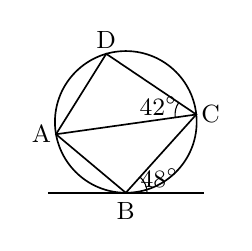
\begin{tikzpicture}[scale=0.9, line width=0.6pt]
  \draw (0.000,0.000) circle (1.000);
  \draw (-1.100,-1.000) -- (1.100,-1.000);
  \draw (-0.985,-0.174) -- (-0.000,-1.000) -- (0.995,0.105) -- (-0.276,0.961) -- cycle;
  \draw (-0.985,-0.174) -- (0.995,0.105);
  \draw[line width=0.4pt] (0.746,0.272) arc[start angle=146.000, end angle=188.000, radius=0.300];
  \node[font=\small, inner sep=1pt] at (0.459,0.228) {$42^\circ$};
  \draw[line width=0.4pt] (0.300,-1.000) arc[start angle=0.000, end angle=48.000, radius=0.300];
  \node[font=\small, inner sep=1pt] at (0.475,-0.788) {$48^\circ$};
  \node[font=\small, anchor=east, inner sep=1.5pt] at (-0.985,-0.174) {A};
  \node[font=\small, anchor=north, inner sep=1.5pt] at (-0.000,-1.060) {B};
  \node[font=\small, anchor=west, inner sep=1.5pt] at (0.995,0.105) {C};
  \node[font=\small, anchor=south, inner sep=1.5pt] at (-0.276,0.961) {D};
\end{tikzpicture}
}{% 0574(본책 103쪽) 보기 ② — 점 T 에서 외접하는 두 원, 공통 접선 PQ, 직선 ATC·BTD, 현 AB·CD. 스캔 삽화를 TikZ 로 다시 그림.
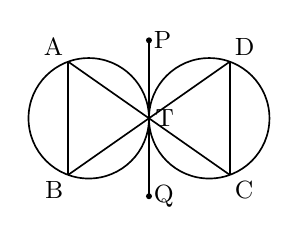
\begin{tikzpicture}[scale=0.9, line width=0.6pt]
  \draw (-0.850,0.000) circle (0.850);
  \draw (0.850,0.000) circle (0.850);
  \draw (0.000,1.100) -- (0.000,-1.100);
  \fill (0.000,1.100) circle (1.2pt);
  \fill (0.000,-1.100) circle (1.2pt);
  \draw (-1.141,0.799) -- (1.141,-0.799);
  \draw (-1.141,-0.799) -- (1.141,0.799);
  \draw (-1.141,0.799) -- (-1.141,-0.799);
  \draw (1.141,-0.799) -- (1.141,0.799);
  \node[font=\small, anchor=south east, inner sep=1.5pt] at (-1.141,0.819) {A};
  \node[font=\small, anchor=north east, inner sep=1.5pt] at (-1.141,-0.819) {B};
  \node[font=\small, anchor=north west, inner sep=1.5pt] at (1.141,-0.819) {C};
  \node[font=\small, anchor=south west, inner sep=1.5pt] at (1.141,0.819) {D};
  \node[font=\small, anchor=west, inner sep=1.5pt] at (0.020,0.000) {T};
  \node[font=\small, anchor=west, inner sep=1.5pt] at (0.000,1.100) {P};
  \node[font=\small, anchor=west, inner sep=1.5pt] at (0.000,-1.100) {Q};
\end{tikzpicture}
}{% 0574(본책 103쪽) 보기 ③ — 두 점 P·Q 에서 만나는 두 원, 직선 APD·BQC, 현 AB·CD. 스캔 삽화를 TikZ 로 다시 그림.
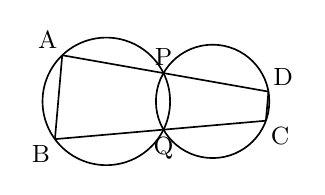
\begin{tikzpicture}[scale=0.9, line width=0.6pt]
  \draw (-0.750,0.000) circle (0.900);
  \draw (0.750,0.000) circle (0.800);
  \draw (-1.372,0.651) -- (1.538,0.138);
  \draw (-1.475,-0.533) -- (1.502,-0.273);
  \draw (-1.372,0.651) -- (-1.475,-0.533);
  \draw (1.502,-0.273) -- (1.538,0.138);
  \node[font=\small, anchor=south east, inner sep=1.5pt] at (-1.372,0.671) {A};
  \node[font=\small, anchor=north east, inner sep=1.5pt] at (-1.475,-0.553) {B};
  \node[font=\small, anchor=north west, inner sep=1.5pt] at (1.502,-0.293) {C};
  \node[font=\small, anchor=south west, inner sep=1.5pt] at (1.538,0.158) {D};
  \node[font=\small, anchor=south, inner sep=1.5pt] at (0.057,0.439) {P};
  \node[font=\small, anchor=north, inner sep=1.5pt] at (0.057,-0.439) {Q};
\end{tikzpicture}
}{% 0574(본책 103쪽) 보기 ④ — 두 점 P·Q 에서 만나는 두 원, 직선 APD·BQC, 현 AB·CD, PC·QD. 스캔 삽화를 TikZ 로 다시 그림.
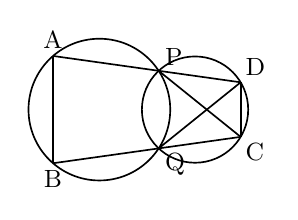
\begin{tikzpicture}[scale=0.9, line width=0.6pt]
  \draw (-0.800,0.000) circle (1.000);
  \draw (0.550,0.000) circle (0.750);
  \draw (-1.454,0.757) -- (1.194,0.385);
  \draw (-1.454,-0.757) -- (1.194,-0.385);
  \draw (-1.454,0.757) -- (-1.454,-0.757);
  \draw (1.194,-0.385) -- (1.194,0.385);
  \draw (0.037,0.547) -- (1.194,-0.385);
  \draw (0.037,-0.547) -- (1.194,0.385);
  \node[font=\small, anchor=south, inner sep=1.5pt] at (-1.454,0.787) {A};
  \node[font=\small, anchor=north, inner sep=1.5pt] at (-1.454,-0.787) {B};
  \node[font=\small, anchor=north west, inner sep=1.5pt] at (1.194,-0.405) {C};
  \node[font=\small, anchor=south west, inner sep=1.5pt] at (1.194,0.405) {D};
  \node[font=\small, anchor=south west, inner sep=1.5pt] at (0.057,0.547) {P};
  \node[font=\small, anchor=north west, inner sep=1.5pt] at (0.057,-0.547) {Q};
\end{tikzpicture}
}{% 0574(본책 103쪽) 보기 ⑤ — 점 T 에서 내접하는 두 원, 공통 접선 PQ, 직선 TDA·TCB, 현 AB·DC. 스캔 삽화를 TikZ 로 다시 그림.
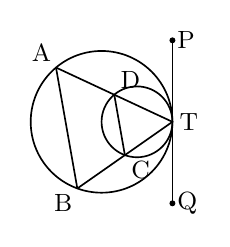
\begin{tikzpicture}[scale=0.9, line width=0.6pt]
  \draw (0.000,0.000) circle (1.000);
  \draw (0.500,0.000) circle (0.500);
  \draw (1.000,1.150) -- (1.000,-1.150);
  \fill (1.000,1.150) circle (1.2pt);
  \fill (1.000,-1.150) circle (1.2pt);
  \draw (1.000,0.000) -- (-0.643,0.766);
  \draw (1.000,0.000) -- (-0.342,-0.940);
  \draw (-0.643,0.766) -- (-0.342,-0.940);
  \draw (0.329,-0.470) -- (0.179,0.383);
  \node[font=\small, anchor=south east, inner sep=1.5pt] at (-0.643,0.786) {A};
  \node[font=\small, anchor=north east, inner sep=1.5pt] at (-0.342,-0.960) {B};
  \node[font=\small, anchor=north west, inner sep=1.5pt] at (0.349,-0.490) {C};
  \node[font=\small, anchor=south west, inner sep=1.5pt] at (0.199,0.403) {D};
  \node[font=\small, anchor=west, inner sep=1.5pt] at (1.030,0.000) {T};
  \node[font=\small, anchor=west, inner sep=1.5pt] at (1.000,1.150) {P};
  \node[font=\small, anchor=west, inner sep=1.5pt] at (1.000,-1.150) {Q};
\end{tikzpicture}
}\end{choicesii}
